%&pdflatex
\documentclass{article}
\usepackage[utf8]{inputenc}

% Set page geometry.
\usepackage{geometry}
 \geometry{
 a4paper,
 total={170mm,257mm},
 left=20mm,
 top=10mm,
 }

% Packages for maths symbols.
\usepackage{amsmath}
\usepackage{amsfonts}
\usepackage{graphicx}
\usepackage[colorlinks=true, allcolors=blue]{hyperref}
\usepackage{xcolor}
\usepackage{tikz}
\usepackage{pgfplots}

% Various definitions.
%\definecolor{bblue}{rgb}{0.36, 0.54, 0.66}
\def \Z {\mathbb{Z}}
\def \N {\mathbb{N}}
\def \Q {\mathbb{Q}}
\def \R {\mathbb{R}}
\def \C {\mathbb{C}}
\def \E {\mathbb{E}}
\def \P {\mathbb{P}}
\def \> {\Rightarrow}
%\def \bb {\color{bblue}}
\def \thm {\par \begingroup \narrower \noindent}
\def \thmend {\par \endgroup}
\def \x {\textbf{x}}
\def \y {\textbf{y}}


% Document Specifics.
\author{William A. Bevington}
\title{Analysis Hand in Three}
\date{}
\begin{document}
\maketitle
%%%%%%%%%%%%%%%%%%%%%%%%%%%%%%%%%%%%%%%%%%%%%%%%%%%%%%%%%%%%%%%%%%%%%%%%%%%%%%%%
\section*{Question One - Workshop 6, Q6}
\subsection*{Part A}
So we have the three metrics on $\R^2$ given by:
	\[
		d_1(\x,\y) := \sum_{k=1}^n |x_k-y_k|, \quad
		d_2(\x,\y) := |\x-\y|, \quad
		d_\infty(\x,\y) := \max_{1\leq k\leq n}|x_k-y_k|.
	\]

Below we have plots of the unit balls centered at the origin with the {\color{red}$d_1$ metric}, the {\color{blue}$d_2$ metric} and the {\color{green}$d_\infty$ metric} on the left. On the right I've added a ball of radius two in the {\color{orange} $d_1$ metric}, centered at the origin.

\begin{centering}
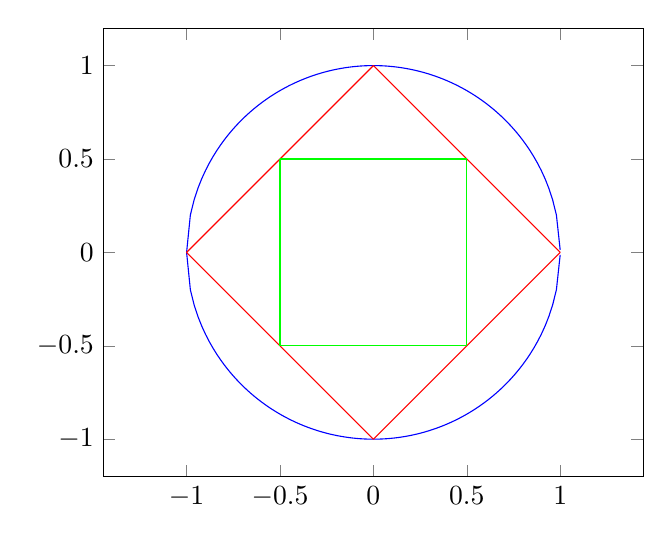
\begin{tikzpicture}
\begin{axis}[axis equal]
%For the metric d_2
	\addplot
	[domain=-1:1,
	samples=100,
	color=blue,]{sqrt( 1 - x^2 )};
	\addplot 
	[domain=-1:1,
	samples=100,
	color=blue,]{-sqrt( 1 - x^2 )};
%%%%%%%%%
%For the metric d_1
	\addplot 
	[domain=0:1,
	samples=100,
	color=red,]{1-x};
	\addplot
	[domain=-1:0,
	samples=100,
	color=red,]{1+x};
	\addplot
	[domain=0:1,
	samples=100,
	color=red,]{-1+x};
	\addplot 
	[domain=-1:0,
	samples=100,
	color=red,]{-1-x};
%%%For the metric d_\infty
	\addplot
	[domain=-0.5:0.5,
	samples=100,
	color=green,]{0.5};
	\addplot 
	[domain=-0.5:0.5,
	samples=100,
	color=green,]{-0.5};
	\addplot 
	[domain=-0.5:0.5,
	samples=100,
	color=green,]({0.5},{x});
	\addplot
	[domain=-0.5:0.5,
	samples=100,
	color=green,]({-0.5},{x});
\end{axis}
\end{tikzpicture}
%
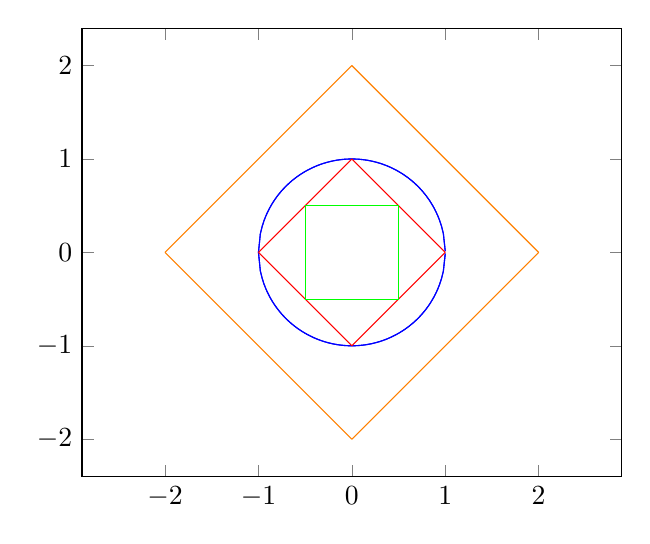
\begin{tikzpicture}
\begin{axis}[axis equal]
	\addplot
	[domain=0:2,
	samples=100,
	color=orange,]{2-x};
	\addplot 
	[domain=-2:0,
	samples=100,
	color=orange,]{2+x};
	\addplot 
	[domain=0:2,
	samples=100,
	color=orange,]{-2+x};
	\addplot 
	[domain=-2:0,
	samples=100,
	color=orange,]{-2-x};
%For the metric d_2
	\addplot 
	[domain=-1:1,
	samples=100,
	color=blue,]{sqrt( 1 - x^2 )};
	\addplot 
	[domain=-1:1,
	samples=100,
	color=blue,]{-sqrt( 1 - x^2 )};
%For the metric d_2
	\addplot
	[domain=-1:1,
	samples=100,
	color=blue,]{sqrt( 1 - x^2 )};
	\addplot 
	[domain=-1:1,
	samples=100,
	color=blue,]{-sqrt( 1 - x^2 )};
%%%%%%%%%
%For the metric d_1
	\addplot 
	[domain=0:1,
	samples=100,
	color=red,]{1-x};
	\addplot
	[domain=-1:0,
	samples=100,
	color=red,]{1+x};
	\addplot
	[domain=0:1,
	samples=100,
	color=red,]{-1+x};
	\addplot 
	[domain=-1:0,
	samples=100,
	color=red,]{-1-x};
%%%For the metric d_\infty
	\addplot
	[domain=-0.5:0.5,
	samples=100,
	color=green,]{0.5};
	\addplot 
	[domain=-0.5:0.5,
	samples=100,
	color=green,]{-0.5};
	\addplot 
	[domain=-0.5:0.5,
	samples=100,
	color=green,]({0.5},{x});
	\addplot
	[domain=-0.5:0.5,
	samples=100,
	color=green,]({-0.5},{x});
\end{axis}
\end{tikzpicture}
\end{centering}


\subsection*{Part B}
We must show first that $d_\infty(\x,\y)\leq d_2(\x,\y)$, that is, that $\max_{1\leq k \leq 2}|x_k-y_k| < |\x-\y|$. So for any $\x$ and $\y$ we have that $d_\infty(\x,\y) = \max_{1\leq k \leq 2}|x_k-y_k| = |x_j-y_j|$ for some $j$, and that $d_2(\x,\y) = \sqrt{(x_1-y_1)^2+(x_2-y_2)^2}$. Note that $(d_2(\x,\y))^2 = (x_1-y_1)^2+(x_2-y_2)^2 \geq (x_i-y_i)^2$ for any $i$ by the triangle inequality, so for any $i,j$ we have that
	\begin{align*}
		d_2(\x,\y)^2 &\geq |x_j-y_j|^2 \\
		\Rightarrow
		d_2(\x,\y)   &\geq |x_j-y_j|
	\end{align*}
and so $d_2(\x,\y)\geq d_\infty(\x,\y)$

Now we need to show that $d_2(\x,\y)\leq d_1(\x,\y)$, in other words we need to show that $\sqrt{(x_1-y_1)^2+(x_2-y_2)^2} \leq \sum_{k=0}^n |x_k-y_k| = |x_1-y_1| + |x_2-y_2|$. Note that $a^2+b^2 \leq (a+b)^2=a^2+b^2+2ab$ in general (for $a,b\geq0$), so letting $a=|x_1-y_1|>0$ and $b=|x_2-y_2|>0$ we get
	\begin{align*}
		|x_1-y_1|^2+|x_2-y_2|^2 &\leq (|x_1-y_1|+|x_2-y_2|)^2 \\
		\Rightarrow
		\sqrt{|x_1-y_1|^2+|x_2-y_2|^2} &\leq |x_1-y_1|+|x_2-y_2|\\
		\Rightarrow
		d_2(\x,\y) &\leq d_1(\x,\y)
	\end{align*}
which is what we wanted, though we've only proved this for $\R^2$, but that's all that's required.

Finally we must show that $d_1(\x,\y)\leq nd_\infty(\x,\y)$. By definition of $d_\infty(\x,\y)$, for any $i$ we have that if $d_\infty(\x,\y)=|x_a-y_a|$ then $|x_i-y_i|\leq|x_a-y_a|$. So we have that 
	\begin{align*}
		d_1(\x,\y):=\sum_{i=1}^n |x_i-y_i| &\leq \sum_{i=1}^n |x_a-y_a| \\
		&= n|x_a-y_a| \\
		&= nd_\infty(\x,\y)
	\end{align*}
and so we have finally that
	\[
		d_\infty(\x,\y) \leq d_2 (\x,\y)\leq d_1 (\x,\y)\leq nd_\infty(\x,\y).
	\]
Looking at our plots in part a we see that this is true at least in the case $n=2$.

\subsection*{Part C}
This is just an application of the Cauchy-Schwarz inequality:
	\begin{align*}
		\sum_{k=1}^n a_kb_k &\leq \sqrt{\sum_{k=1}^na_k^2}\sqrt{\sum_{k=1}^nb_k^2} \\
		\Rightarrow \left(\sum_{k=1}^na_k\right)^2 &\leq n\sum_{k=1}^na_k^2
	\end{align*}
by letting $b_i=1$ for all $i$ and squaring both sides. This gives us that $\sum_{k=1}^n|x_k-y_k| \leq \sqrt{n}\sqrt{(x_1-y_1)^2 + (x_2-y_2)^2}$, and so $d_1(\x,\y) \leq \sqrt{n} d_2(\x,\y)$, and we are done.

Let $d_\infty(\x,\y) := \max_{1\leq i\leq n}|x_i-y_i| = |x_k-y_k|$ for some $1\leq k\leq n$, then for any $i\in\{1,\dots,n\}$ we have that $|x_i-y_i|^2\leq|x_k-y_k|^2$, which gives us that $\sum_{i=1}^n|x_i-y_i|^2\leq n|x_k-y_k|^2$ and so $\sqrt{\sum_{i=1}^n|x_i-y_i|^2} \leq \sqrt{n}\sqrt{|x_k-y_k|^2}$, but this is just saying that $d_2(\x,\y) \leq \sqrt{n}d_\infty(\x,\y)$ so we are done.



%%%%%%%%%%%%%%%%%%%%%%%%%%%%%%%%%%%%%%%%%%%%%%%%%%%%%%%%%%%%%%%%%%%%%%%%%%%%%%%%
\section*{Question Two Workshop 6, Q7a}
%What conditions ensure $g:[0,\infty)\to\R$, $p(x,y):=g(|x-y|)$ is a metric?

If $f:\R\to\R$ then the form $d(x,y) := |f(x)-f(y)|$ is a metric if
\begin{enumerate}
	\item $d(x,x) = |f(x)-f(x)| = 0$
	\item $d(x,y) = |f(x)-f(y)| > 0$ if $x\neq y$
	\item $d(x,y) = d(y,x)$
	\item $d(x,z) \leq d(x,y) + d(y,z)$
\end{enumerate}

Criteria one and three are satisfied automatically if $f$ is well-defined, since $|f(x)-f(x)|=0$ and $|f(x)-f(y)|=|f(y)-f(x)|$, so we need only find criteria for when two and four are satisfied. $|f(x)-f(y)|=0\Rightarrow x=y$, is satisfied iff $f(x)=f(y) \Rightarrow x=y$, ie, when $f$ is injective.

We wish to find out when $|f(x) - f(z)| \leq |f(x) - f(y)| + |f(y)-f(z)|$. This is simply inherited from $\R$ for suitable $f$, so we only have to worry about the values $a$ for which $f(a)\notin\R$. This only happens if  $\lim_{x\to a} f(x) =\pm\infty$ at $a$. Here it might be the case that $|f(a)-f(y)|>|f(a)-f(z)|+|f(z)-f(y)|$, so we require that $f$ is never infinite, that is; $f$ bounded. Thus $f$ being bounded, well-defined and injective are necessary and sufficient conditions for $d(x,y):=|f(x)-f(y)|$ to be a metric.


\end{document}
